\documentclass[UTF8, 11pt, oneside]{ctexart}

\usepackage{float}

\usepackage{geometry}
\geometry{a4paper,left=2cm,right=2cm,top=2cm,bottom=1cm}

\usepackage{graphicx}

\usepackage{hyperref}
\hypersetup{colorlinks=true, linkcolor=red}

\linespread{1.6}


\def\articletitle{古有族田义庄,今有家族基金,国有义务教育}

\usepackage{fancyhdr}
\usepackage{ifthen}
\pagestyle{fancy}
\fancyhf{}
\setlength{\headheight}{14pt}
\fancyhead[R]{\ifthenelse{\value{page}>1}{\thepage}{}}
\fancyhead[C]{\ifthenelse{\value{page}>1}{\articletitle}{}}
\renewcommand\headrulewidth{0pt}

\usepackage{tcolorbox}
\tcbuselibrary{skins}


\newcommand{\zd}[1]{\textbf{\textcolor[RGB]{123,12,0}{#1}}} % 重点

\newcommand{\yh}[1]{% 引用
    \begin{tcolorbox}[enhanced,
        frame hidden, interior hidden,
        before skip = 5mm, left skip=10mm,
        borderline west={5pt}{0pt}{gray!50}]
        #1
    \end{tcolorbox}
}

\newcommand{\biaoti}[1]{% 标题
    \section*{#1}
}

\begin{document}

\begin{center}
    \LARGE{\articletitle\footnotemark}
\end{center}
\footnotetext{
    原文出自公众号“远方青木”的文章 《\href{https://mp.weixin.qq.com/s/cPQgG9JJVY2M5sLwukC1SA}{\articletitle}》
}

如何传承一个家族的财富?

北宋的范仲淹,给出了一个最完美的答案。

那位说出“先天下之忧而忧,后天下之乐而乐”这句千古名言的范仲淹。

宋仁宗皇佑二年(1050),时任杭州太守的范仲淹宣布捐出他一生的全部积蓄,在苏州购置了1000多亩良田,专为范氏宗族所用。

\zd{这大概是人类历史上最早的家族基金会了,今天欧美富豪玩的那一套,近千年前范仲淹就发明了。}

范仲淹将这千亩良田,划归给“\zd{范氏义庄}”,并亲自制定范氏义庄的规章制度。

一、口粮:五岁以上的范氏各房族人,不分男女,每口每月给白米三斗。

二、衣料:成年族人每人每年给冬衣衣料一匹;十岁以下、五岁以上的儿童各给半匹。

三、婚姻补助:族人嫁女,给钱三十贯;女儿若改嫁,给钱二十贯;族人娶媳妇,给钱二十贯,二婚不给钱。

四、丧葬费:族人身亡,按其辈份大小,给予二贯至二十五贯的安葬费。

五、路费:族人参加科举,或者外出赴任,给予路费补助。

范仲淹还另外规定:

倘若乡亲、姻亲、亲戚陷入贫困,或遇饥荒不能生存时,诸房共同核实后,可用义庄粮米“量行济助”。

为确保义庄土地不会被后世子孙所糟蹋,范仲淹规定义庄的田地屋舍不得出售,平时由人独立掌管,全族监督,但即便是族长,也不得干预掌管人依规办事,为杜绝贪污,范仲淹甚至不允许族人借用义庄的人力、车、船和器用。

否则,以大不孝论处。

除此之外,为了保证义庄的义这个字。

范氏义庄不得使用本族族人作为义田的佃户,不得典买本族族人的土地。

\zd{换句话说,就是不准内卷,只准外卷。}

有了范氏义庄后,可以说所有范氏的族人都有了一个保底的生存条件和基本的婚嫁体面,然后族人们通过源源不断的教育不断的诞生新的精英。

\zd{范仲淹此举,可谓是为自家宗族立下了万世之基。}

\begin{figure}[H]
    \centering
    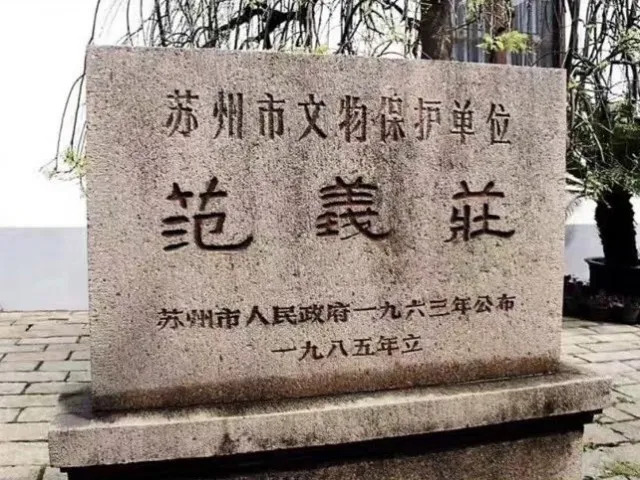
\includegraphics[width=10cm]{2024-03-20-001}
\end{figure}

在千年时间里,周边的宗族消失了一个又一个,但范氏宗族始终长盛不衰。

宋朝,范氏宗族中进士者22人,明朝中进士者30人,清朝仅顺治时期就出进士12人。

到了清末,因为每一个优秀族人不断的捐赠,范氏的义田规模已经达到了5300亩的巅峰。

每一个进士的出现,都让范氏宗族成为了周边都不敢惹的霸主存在。

但偏偏范氏一族的进士可谓是连绵不断,让宗族得以\zd{辉煌千年}。

宋朝有很多人比范仲淹有钱,也有不少人比范仲淹官大。

但能让自家宗族辉煌千年的,几乎一个都没有。

千年时光实在太漫长了,没人能保证自家不出败家子,哪怕皇帝都没这个本事。

但范仲淹做到了这个奇迹。

因为义田的所有权属于宗族,不属于任何人,所以义田又被称之为族田。

\zd{族田的一切产出,都为族人共有。}

\zd{相当于本族人的社保。}

利于一切族人,但因为是接近于平均分配,对穷苦族人更为重要,对于富贵族人而言用途很小。

历朝历代,耕读世家都是传递血脉的不二法宝,利用土地做保底收入,利用大量后代博概率出精英。

卖祖田肯定是被禁止的,而且一定是写入家规的。

\zd{但不管你把祖田传给谁,都一定会在某一代产生一个败家子,禁是禁不住的。}

\zd{但范仲淹的这种族田方式,全族共有,没有人拥有实际所有权。}

有人想卖田,需要说服全族所有人,卖的钱也不归自己拿,而是归全族所有人共有。

这种极度困难且自己没啥好处的事情,就没人愿意干了。

\zd{而只要族田义庄能保留下来,族人们就能有最低的生活保障,时光不再是磨灭宗族的敌人,而是朋友。}

族田义庄一经发明,很快就被很多宗族所采纳。

1949年,徽州耕地面积是118万亩,其中属于各宗族的族田就有16.9万亩,占徽州总耕地面积的14.32\%。

\zd{很多人不理解为什么解放前各地区宗族的影响力那么大,宗族规矩的威慑力甚至比法律还要大。}

因为宗族拥有如此巨大规模的族田,给所有族人提供低保,那影响力自然很巨大。

而在解放前,官府只负责收税,其他什么都不管。

所以违反了族规,被驱逐出了宗族,后果是非常严重的,比违反当时的法律后果要严重的多。

\begin{figure}[H]
    \centering
    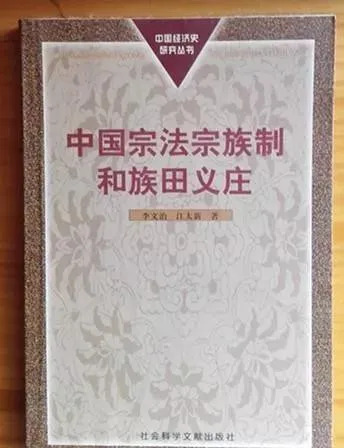
\includegraphics[width=10cm]{2024-03-20-002}
\end{figure}

\zd{置办族田,几乎成了一个宗族的标志物,没有族田就不配称之为宗族。}

后人还在族田的基础上,发明了祭祀田、学田和书田等。

祭祀田就是所有产出专供祭祀的田地。

而学田和书田,顾名思义,就是所有产出专供给族人进行读书所用,相当于宗族举办的免费义务教育。

在古代,皇权不下乡,宗族就是地方上的小政府。

\zd{以族田的产出作为经济支撑,族内的救济穷人,兴办教育,祭祀祖宗等一切公共开支,都由族田出钱。}

\begin{figure}[H]
    \centering
    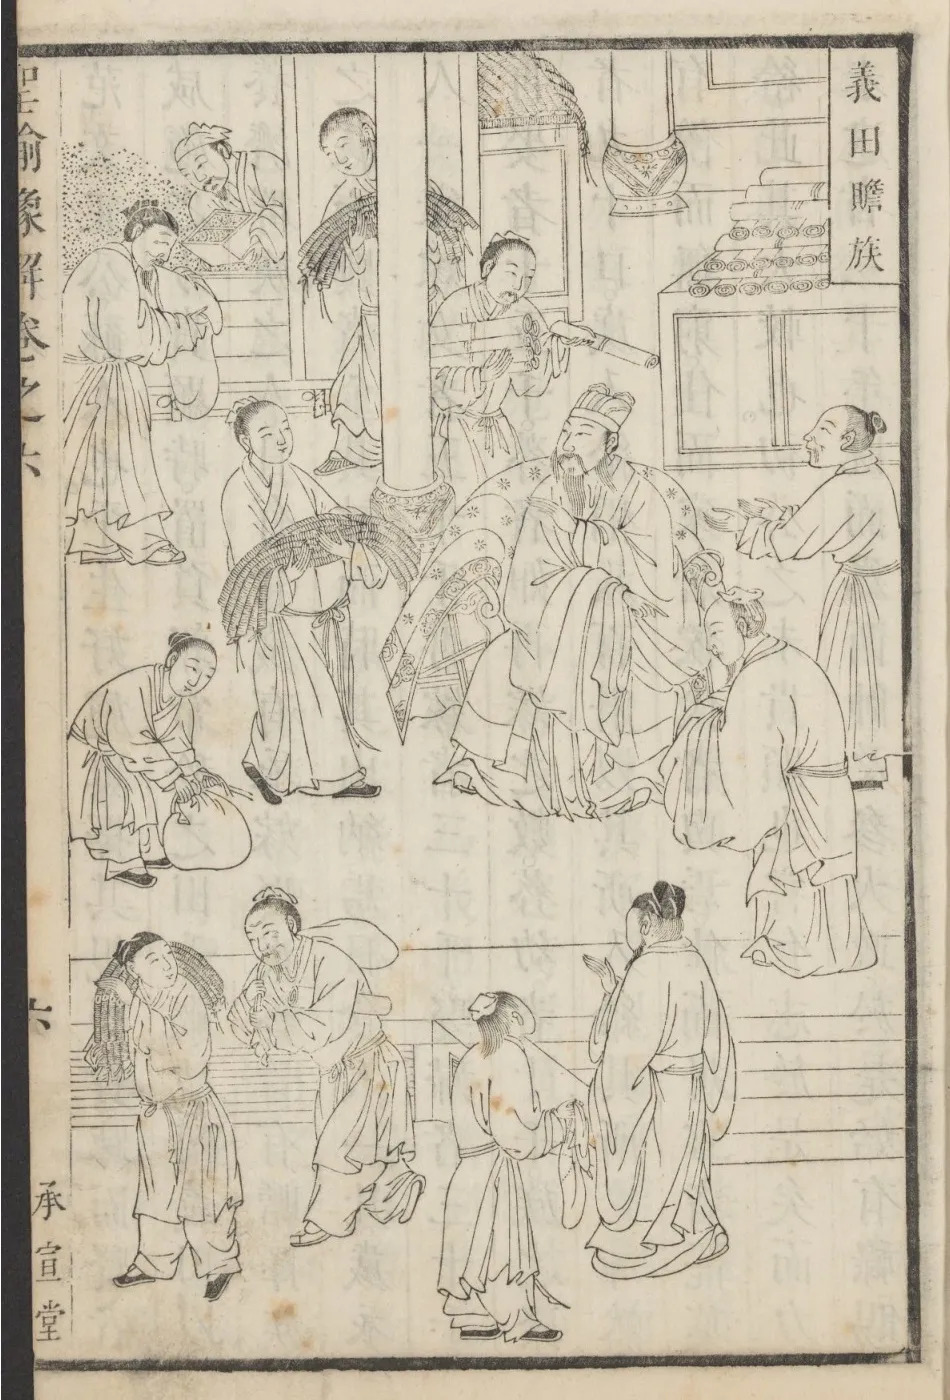
\includegraphics[width=10cm]{2024-03-20-003}
\end{figure}

因此,拥有族田的宗族,才能辉煌千年。

而没有族田的宗族,衰落的非常非常快。

在美国,其实也有类似的操作,那就是家族基金会。

卡耐基金会、洛克菲勒基金会、比尔\&梅琳达·盖茨基金会等等,都是美国富豪为了传承自己的财富而设置的基金会。

其设立初衷,都是假定自己的孩子是败家子,所以只能在基金会里领“低保”。

基金会的目的不是让某一代孩子奢靡无边,而是让代代孩子都能过上体面的生活。

\zd{富豪更在意自己的血脉能不能永远流传,不在意,甚至要坚决禁止孩子们的奢靡生活。}

没有任何族人能卖族田,也没有任何富豪后代能卖掉家族基金会的财产。

两者的相似性是很大的。

但不同之处也很大。

美国的家族基金会,只会照顾自己的后人,不会去照顾自己远房亲戚的孩子,也没有宗族一说。

而范仲淹的制度,能被称之为义庄,那是名副其实。

因为范仲淹要照顾的,不仅是自己的后人,还有自己的全族之人。

\zd{从初衷上,范仲淹的义庄制度,要比家族基金会高大太多。}

\zd{而从实际效果上,义庄制度也要好很多,因为义庄制度下出精英的概率要大太多。}

如果美国的富豪们特别能生,每一代生十几个后代,那么几代之后就可以自成一族,两者的区别不会有太大。

但如今的美国,生育率并不高,几代之后总人口可能变化不大,这就导致家族基金会未必保险,很可能会在一段时间后出问题。

族田和义庄之所以能辉煌千年,能持续的供给现金流只是其中原因之一,能让全族代代出人才,这才是最核心的因素。

范氏宗族任何时期都至少有一个进士的存在,而在古代的宗族礼法下,这个进士也必须照顾本族,至少不能让宗族的核心,也就是族田受损,否则全国人都会戳这个进士的脊梁骨,被视为大不孝,哪怕皇帝都会觉得这个人靠不住。

族田供养你成了进士,如今你居然让族田受损而置之不理,这种狼心狗肺的人谁敢用?

这才是周边的豪强在千年时光里都不敢觊觎范氏族田的原因。

\zd{不敢动范氏族田不是因为范氏有钱,而是因为范氏宗族里一直有进士,而且很可能十几年后再出一个新进士。}

这简直太可怕了。

\zd{族田永远有人保护,永远不受损,永远能给族人最低的生活保障,你说这种制度下的范氏宗族,岂能不辉煌。}

如果无人保护族田,那当全族遭遇灭亡危机时,所谓的族田不可卖就是一个笑话。

\zd{族人都快没了,还要族田干嘛。}

美国那边的家族基金会也是一样,基金会的初衷是为了血脉流传,如果血脉都快断了还坚持不给钱,那同样会陷入道德悖论,到时候基金会还是会被卖掉,哪怕饮鸩止渴都得卖。

坚持不卖也没事,血脉断了之后家族基金会失去所有的权益继承人。

那效果和整个基金会被打包卖了送人是一样的,见效还更快,连饮鸩止渴的机会都不给你。

中国族田和美国基金会的出现初衷,都是为了规避最差劲的败家子掌控财产这种情况的出现,期待通过普惠政策,慢慢等候精英后代的出现。

只有源源不断出现的精英后代,才能真正保护族田,才能真正保护所有人的利益。

美国的家族基金会只保护自己的后代,格局低了,不如族田和义庄。

族田和义庄只保护自己宗族之人,其实格局也低了。

\zd{1949年解放后,中国所有的族田和义庄都消失了,取而代之的是国田。}

\zd{而国田,也承担了过去族田和义庄的功能。}

以前的官府,只负责收税,其他一概都不管。

而今天的政府,把接济贫穷,赈恤孤寡和协济国人读书应试,作为自己的主要职责。

\zd{把一国,视为一族。}

然后,对本族之人给与最低生活保障,通过种种手段,让所有人都吃得饱穿得暖。

在能吃饱穿暖的基础上,给与全民义务教育,让每个人都有读书的机会,费用国家来出。

\zd{全民义务教育推行后,每一代,都能出现大量的精英族人。}

然后这些族人,再反过来保护全族的核心利益不受损害。

以前,只有大宗族才能拥有族田,也只有大宗族才能保证一直有精英族人的保护,小族之人只有逐渐衰亡一条路,生存空间会慢慢被大宗族蚕食一空。

而现在,全中国所有人都能享受到以前大宗族的待遇。

\zd{以前是宗族所有人联手对外,现在是全国所有人联手对外。}

这就是为什么旧社会的政府在新中国政府手底下不堪一击的原因。

\zd{中国已经形成了族田的制度,而且是举国为族,生活低保+义务教育已经覆盖到了每一个中国人。}

这个制度,能保证中国全族代代都出精英人才。

培育这些精英人才,是设立族田制度的目的,因为族田制度需要这些精英人才来守护,否则就一定会被外部势力所觊觎,所破坏。

在古代,任由族田受损,宗族核心利益丧失但坐视不管的精英族人,会被所有人看不起,脊梁骨都会被戳断,被视为大不孝。

\zd{今天的中国,自然也是一样。}

\end{document}

